

\tikzset{every picture/.style={line width=0.75pt}} %set default line width to 0.75pt        
\begin{center}
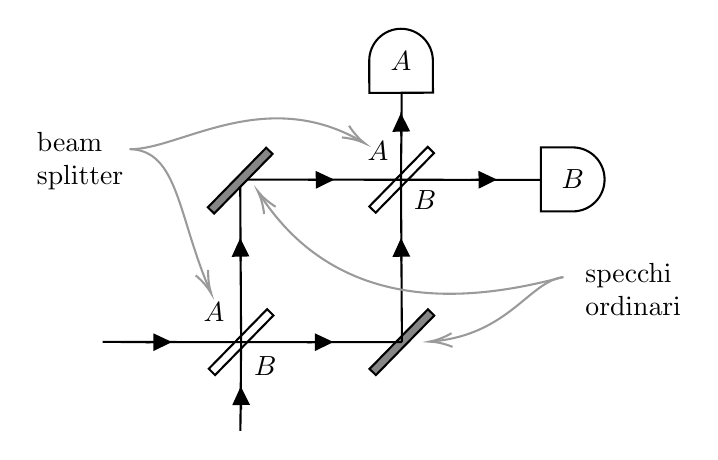
\begin{tikzpicture}[x=0.75pt,y=0.75pt,yscale=-1,xscale=1]
%uncomment if require: \path (0,300); %set diagram left start at 0, and has height of 300

%Shape: Rectangle [id:dp03258470004560032] 
\draw   (314.64,178.14) -- (342.76,149.42) -- (345.8,152.43) -- (317.68,181.15) -- cycle ;
%Straight Lines [id:da6232747865539225] 
\draw    (330.22,165.29) -- (329.88,208) ;


%Straight Lines [id:da7516321880556363] 
\draw    (263.51,165.2) -- (330.22,165.29) ;


%Straight Lines [id:da7431820818677963] 
\draw    (329.78,87.5) -- (330.22,165.29) ;


%Shape: Rectangle [id:dp9234193027203714] 
\draw  [color={rgb, 255:red, 0; green, 0; blue, 0 }  ,draw opacity=1 ][fill={rgb, 255:red, 134; green, 134; blue, 134 }  ,fill opacity=1 ] (392.11,178.18) -- (420.24,149.46) -- (423.28,152.47) -- (395.15,181.19) -- cycle ;
%Shape: Rectangle [id:dp45539842012124043] 
\draw   (392,99.91) -- (420.13,71.19) -- (423.17,74.2) -- (395.05,102.92) -- cycle ;
%Straight Lines [id:da41484953628459365] 
\draw    (330.22,165.29) -- (407.69,165.33) ;


%Straight Lines [id:da6769463633535804] 
\draw    (330.11,87.01) -- (407.59,87.05) ;


%Straight Lines [id:da3686137129912357] 
\draw    (407.25,87.53) -- (407.69,165.33) ;


%Straight Lines [id:da2517530051922354] 
\draw    (407.59,87.05) -- (474.29,87.14) ;


%Straight Lines [id:da24300038090025722] 
\draw    (407.59,44.82) -- (407.25,87.53) ;


%Shape: Rectangle [id:dp1865303790271311] 
\draw  [color={rgb, 255:red, 0; green, 0; blue, 0 }  ,draw opacity=1 ][fill={rgb, 255:red, 134; green, 134; blue, 134 }  ,fill opacity=1 ] (314.19,100.35) -- (342.32,71.63) -- (345.36,74.64) -- (317.23,103.36) -- cycle ;
%Straight Lines [id:da2941942939542457] 
\draw    (284.27,165.35) -- (294.87,165.26) ;
\draw [shift={(296.87,165.24)}, rotate = 539.49] [fill={rgb, 255:red, 0; green, 0; blue, 0 }  ][line width=0.75]  [draw opacity=0] (8.93,-4.29) -- (0,0) -- (8.93,4.29) -- cycle    ;

%Straight Lines [id:da5296598357878515] 
\draw    (330.27,197.87) -- (330.09,188.64) ;
\draw [shift={(330.05,186.64)}, rotate = 448.87] [fill={rgb, 255:red, 0; green, 0; blue, 0 }  ][line width=0.75]  [draw opacity=0] (8.93,-4.29) -- (0,0) -- (8.93,4.29) -- cycle    ;

%Straight Lines [id:da8396982575668597] 
\draw    (330,126.39) -- (329.82,117.17) ;
\draw [shift={(329.78,115.17)}, rotate = 448.87] [fill={rgb, 255:red, 0; green, 0; blue, 0 }  ][line width=0.75]  [draw opacity=0] (8.93,-4.29) -- (0,0) -- (8.93,4.29) -- cycle    ;

%Straight Lines [id:da43067332906978706] 
\draw    (362.08,165.35) -- (372.68,165.26) ;
\draw [shift={(374.68,165.24)}, rotate = 539.49] [fill={rgb, 255:red, 0; green, 0; blue, 0 }  ][line width=0.75]  [draw opacity=0] (8.93,-4.29) -- (0,0) -- (8.93,4.29) -- cycle    ;

%Straight Lines [id:da3506455513682578] 
\draw    (407.47,126.43) -- (407.29,117.2) ;
\draw [shift={(407.25,115.21)}, rotate = 448.87] [fill={rgb, 255:red, 0; green, 0; blue, 0 }  ][line width=0.75]  [draw opacity=0] (8.93,-4.29) -- (0,0) -- (8.93,4.29) -- cycle    ;

%Straight Lines [id:da5029542426839855] 
\draw    (362.52,87.12) -- (373.12,87.02) ;
\draw [shift={(375.12,87.01)}, rotate = 539.49] [fill={rgb, 255:red, 0; green, 0; blue, 0 }  ][line width=0.75]  [draw opacity=0] (8.93,-4.29) -- (0,0) -- (8.93,4.29) -- cycle    ;

%Straight Lines [id:da08573326322161745] 
\draw    (440.94,87.1) -- (451.54,87) ;
\draw [shift={(453.54,86.99)}, rotate = 539.49] [fill={rgb, 255:red, 0; green, 0; blue, 0 }  ][line width=0.75]  [draw opacity=0] (8.93,-4.29) -- (0,0) -- (8.93,4.29) -- cycle    ;

%Straight Lines [id:da9310563696791143] 
\draw    (407.42,66.18) -- (407.24,56.95) ;
\draw [shift={(407.2,54.95)}, rotate = 448.87] [fill={rgb, 255:red, 0; green, 0; blue, 0 }  ][line width=0.75]  [draw opacity=0] (8.93,-4.29) -- (0,0) -- (8.93,4.29) -- cycle    ;

%Flowchart: Delay [id:dp15978253790159513] 
\draw   (474.67,71.47) -- (490.01,71.47) .. controls (498.48,71.47) and (505.34,78.38) .. (505.34,86.89) .. controls (505.34,95.41) and (498.48,102.31) .. (490.01,102.31) -- (474.67,102.31) -- cycle ;
%Flowchart: Delay [id:dp7496896065211829] 
\draw   (391.99,45.21) -- (391.94,29.79) .. controls (391.91,21.28) and (398.75,14.35) .. (407.22,14.32) .. controls (415.69,14.29) and (422.58,21.17) .. (422.61,29.69) -- (422.66,45.11) -- cycle ;
%Curve Lines [id:da1551059930194223] 
\draw [color={rgb, 255:red, 155; green, 154; blue, 154 }  ,draw opacity=1 ]   (485.48,133.93) .. controls (468.93,136.12) and (459.25,161.6) .. (422.63,164.92) ;
\draw [shift={(420.93,165.05)}, rotate = 355.99] [color={rgb, 255:red, 155; green, 154; blue, 154 }  ,draw opacity=1 ][line width=0.75]    (10.93,-3.29) .. controls (6.95,-1.4) and (3.31,-0.3) .. (0,0) .. controls (3.31,0.3) and (6.95,1.4) .. (10.93,3.29)   ;

%Curve Lines [id:da20331933767853982] 
\draw [color={rgb, 255:red, 155; green, 154; blue, 154 }  ,draw opacity=1 ]   (485.48,133.93) .. controls (446.77,144.11) and (378.73,155.6) .. (338.86,93.54) ;
\draw [shift={(338.26,92.59)}, rotate = 417.77] [color={rgb, 255:red, 155; green, 154; blue, 154 }  ,draw opacity=1 ][line width=0.75]    (10.93,-3.29) .. controls (6.95,-1.4) and (3.31,-0.3) .. (0,0) .. controls (3.31,0.3) and (6.95,1.4) .. (10.93,3.29)   ;

%Curve Lines [id:da4920771230228518] 
\draw [color={rgb, 255:red, 155; green, 154; blue, 154 }  ,draw opacity=1 ]   (276.56,72.31) .. controls (299.96,72.86) and (299.78,104.67) .. (315.08,140.14) ;
\draw [shift={(315.79,141.77)}, rotate = 246.07] [color={rgb, 255:red, 155; green, 154; blue, 154 }  ,draw opacity=1 ][line width=0.75]    (10.93,-3.29) .. controls (6.95,-1.4) and (3.31,-0.3) .. (0,0) .. controls (3.31,0.3) and (6.95,1.4) .. (10.93,3.29)   ;

%Curve Lines [id:da3557276256319264] 
\draw [color={rgb, 255:red, 155; green, 154; blue, 154 }  ,draw opacity=1 ]   (276.56,72.31) .. controls (300.08,72.86) and (341.48,41.28) .. (388.42,68.68) ;
\draw [shift={(389.84,69.53)}, rotate = 211.3] [color={rgb, 255:red, 155; green, 154; blue, 154 }  ,draw opacity=1 ][line width=0.75]    (10.93,-3.29) .. controls (6.95,-1.4) and (3.31,-0.3) .. (0,0) .. controls (3.31,0.3) and (6.95,1.4) .. (10.93,3.29)   ;


% Text Node
\draw (341.93,176.77) node   {$B$};
% Text Node
\draw (317.17,150.66) node   {$A$};
% Text Node
\draw (396.2,73.42) node   {$A$};
% Text Node
\draw (418.86,96.76) node   {$B$};
% Text Node
\draw (519.11,139.77) node  [align=left] {specchi\\ordinari};
% Text Node
\draw (252.63,78.09) node  [align=left] {beam\\splitter};
% Text Node
\draw (490.01,86.89) node   {$B$};
% Text Node
\draw (407.27,29.74) node   {$A$};


\end{tikzpicture}
\end{center}